% !TEX TS-program = pdflatex
% !TEX encoding = IsoLatin

%% Version 4x3 und 16x9  2.2 02.01.2014

% ==== wrapper class ==========================================================
\documentclass[% wrapper-class ETHpres option inspite of aspectratio for beamer-classe
    fourtothree=true, % true (default) -- 4:3-format, false -- 16:9-format
    DepLogo=true      % true -- use deplogo_13.pdf, false (default)
                      %         do not use deplogo_13.pdf for footer
    ]{include/ETHpres}

% ==== misc: you may use or not ===============================================
%\usepackage{graphicx}   % for including figures
%%\graphicspath{{pictures/}}
%\usepackage{tabularx}   % for special table environment (tabularx-table)
%\usepackage{booktabs}   % for table layout
%\usepackage{natbib}     % for bibliography with astron-style
%\bibliographystyle{astron}
%\usepackage{siunitx}    % to use for international units in the real world
%\usepackage[
%    colorlinks=true, linkcolor=white, urlcolor=white, % this is special for this presentation here to get the toc in white
%    hypertexnames=false,% for correct links (duplicate-error solution)
%	setpagesize=false,  % necessary in order to not change text-/paperformat for the document
%	pdfborder={0 0 0},  % removes border around links
%	pdfpagemode=FullScreen,% open pdf in full screen mode
%    pdfstartview=Fit    % fit page to pdf viewer
%]{hyperref}% all links stay black and are thus invisible

% ==== language ================================================================
\usepackage[latin1]{inputenc}
%\usepackage[utf8]{inputenc}
% English
\usepackage[english]{babel}
\AtBeginDocument{\renewcaptionname{english}{\contentsname}{\large Outline}}% toc-name
%% Deutsch
%\usepackage[ngerman]{babel}
%\AtBeginDocument{\renewcaptionname{ngerman}{\contentsname}{\large �bersicht}}% toc-name

% ==== choose the basic color for your presentation ===========================
% colorbar-color
\colorlet{firstcolor}{white} % see pages 2  and 3 of this sample presentation
% bachground color titlepage
\colorlet{secondcolor}{white} % see pages 2  and 3 of this sample presentation

\usepackage{amsmath}
\usepackage{algorithm}
\usepackage[noend]{algpseudocode}

% === fill in first information for the presentation ==========================
\newcommand*{\ETHtitle}{Creating wallpapers using mobile phone photos}
\newcommand*{\ETHauthor}{Seonwook Park}
\newcommand*{\ETHdate}{26.6.2015}
\begin{document}
% =========== begin of titlepage ============
\ETHtitelbild\textcolor{black}{\large\textbf{\ETHtitle}}
\newline
%%
% ==== start here with the text on the titlepage
%%
\textcolor{black}{\tiny{A semester project by Seonwook Park \\[-1.2mm]
Supervised by Michael Gygli and Dengxin Dai}}
\clearpage

\ETHminimal
\textbf{Outline\\}
\begin{itemize}
\item Introduction
\item Method
\begin{itemize}
	\item Suitability: Datasets, Training
	\item Cropping: Saliency, Features, Datasets
\end{itemize}
\item Results and Analysis
\item Summary
\item Further work
\end{itemize}
\clearpage

\ETHminimal
\textbf{Introduction\\}
\newline
\begin{minipage}{0.65\textwidth}
\begin{itemize}
	\item A mobile phone photo gallery contains a variety of images.
	\item Could use photos as wallpapers.
	\item Two challenges: Suitability and Cropping.
\end{itemize}
\end{minipage}
\begin{minipage}{0.4\textwidth}
	\begin{tikzpicture}[remember picture,overlay]
	  \node [xshift=-2.2cm,yshift=-4.1cm] at (current page.north east)
	    {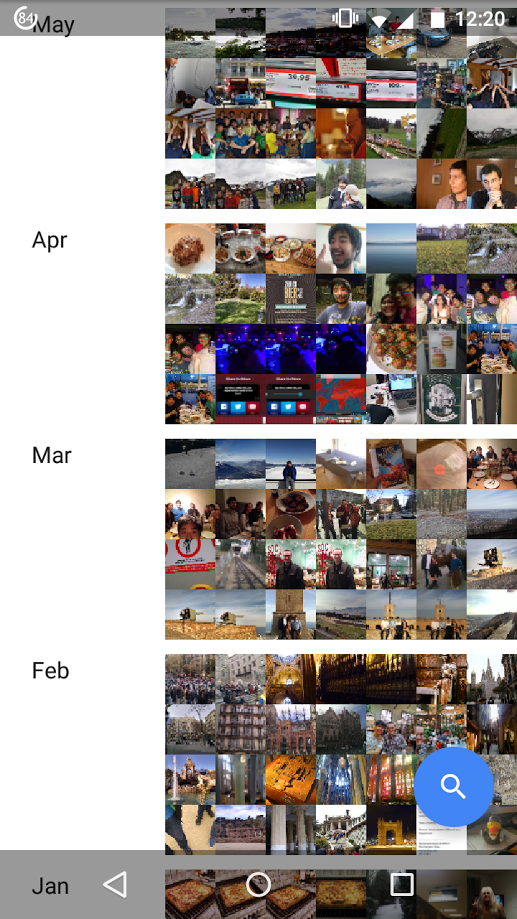
\includegraphics[width=3.2cm]{figures/mobile_gallery.png}};
	\end{tikzpicture}
\end{minipage}
\vspace{16mm}
\begin{itemize}
	\item Which image is suitable as a wallpaper?
	\item Which portion of a selected image should be visible?
\end{itemize}
\clearpage

\ETHminimal
\textbf{Method: Suitability - Datasets\\}
\newline
\begin{minipage}{0.65\textwidth}
\begin{itemize}
	\item Two datasets:
	\begin{itemize}
		\item Michael (275 images)
		\item Wookie (266 images)
	\end{itemize}
	\item Includes:
	\begin{itemize}
		\item Natural scenes
		\item Cityscapes
		\item Short-term memory
		\item Quick photos for messaging
	\end{itemize}
\end{itemize}
\end{minipage}
\begin{minipage}{0.4\textwidth}
	\begin{tikzpicture}[remember picture,overlay]
	  \node [xshift=-1.9cm,yshift=-4.8cm] at (current page.north east)
	    {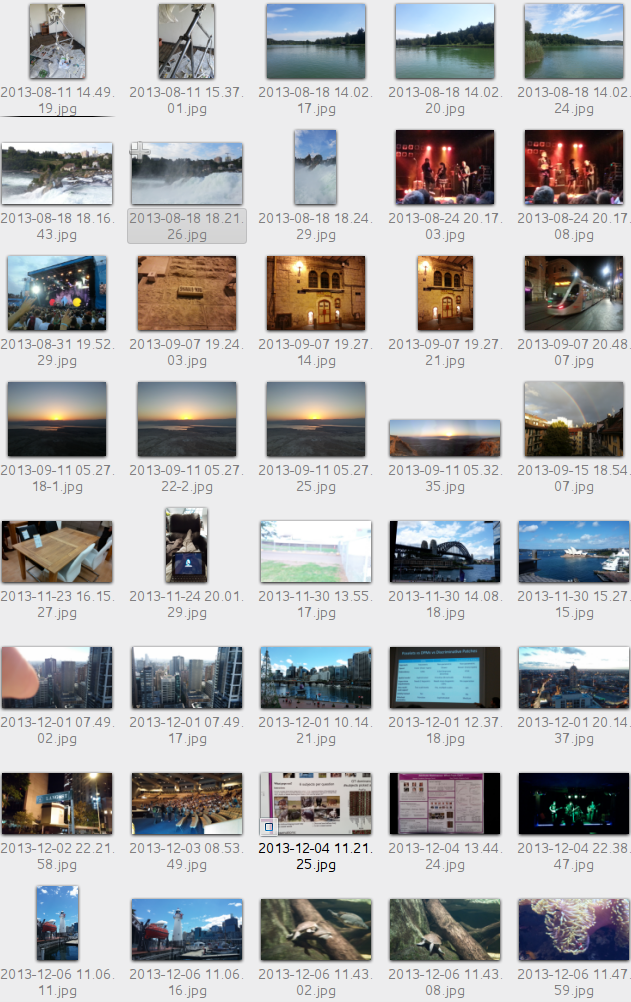
\includegraphics[width=2.9cm]{figures/michael_dataset.png}};
	\end{tikzpicture}
\end{minipage}
\clearpage

\ETHminimal
\textbf{Method: Suitability - Training\\}
\newline
\begin{figure}[h!]
\centering\includegraphics[width=11.5cm]{../figures/pipeline_suitability.pdf}
\end{figure}
\begin{itemize}
	\item Model used: BVLC Reference CaffeNet, 1000 object classes.
\end{itemize}
\clearpage

\ETHminimal
\textbf{Method: Cropping - Saliency}
\begin{figure}[h!]
\centering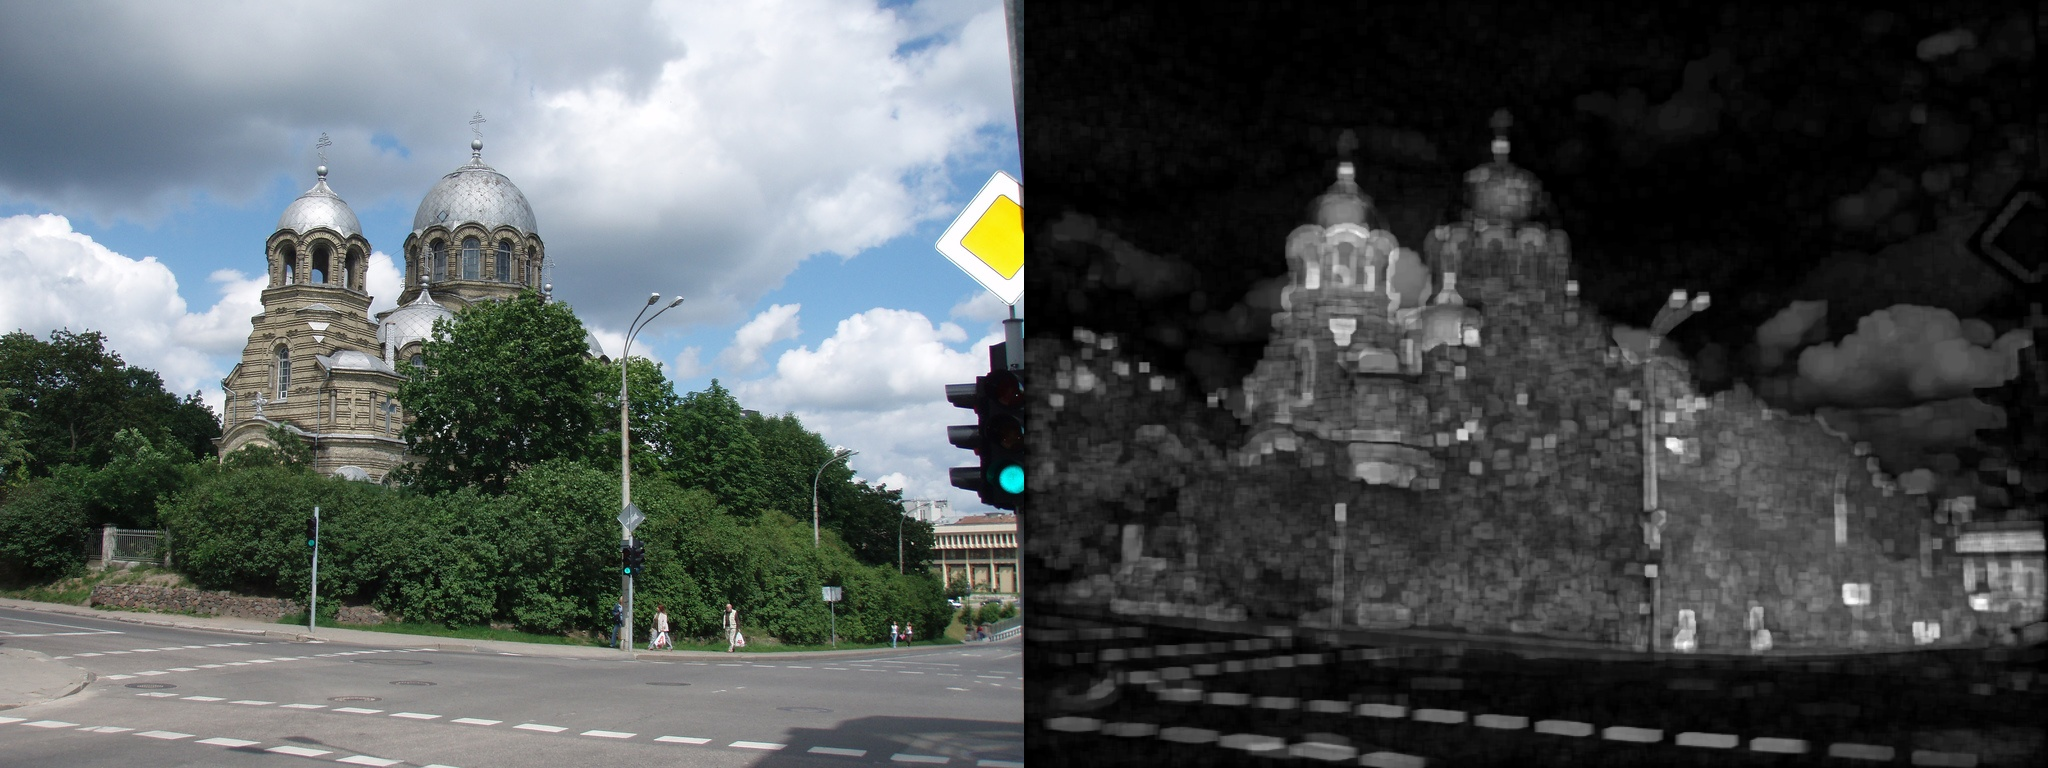
\includegraphics[width=11.5cm]{../figures/example_saliency.jpg}
\end{figure}
\begin{itemize}
	\item Saliency is distinctness compared to neighbouring regions.
	\item Boolean Map based Saliency (BMS) by Zhang et al.
\end{itemize}
\clearpage

\ETHminimal
\textbf{Method: Cropping - Features\\}
\begin{figure}[h!]
\centering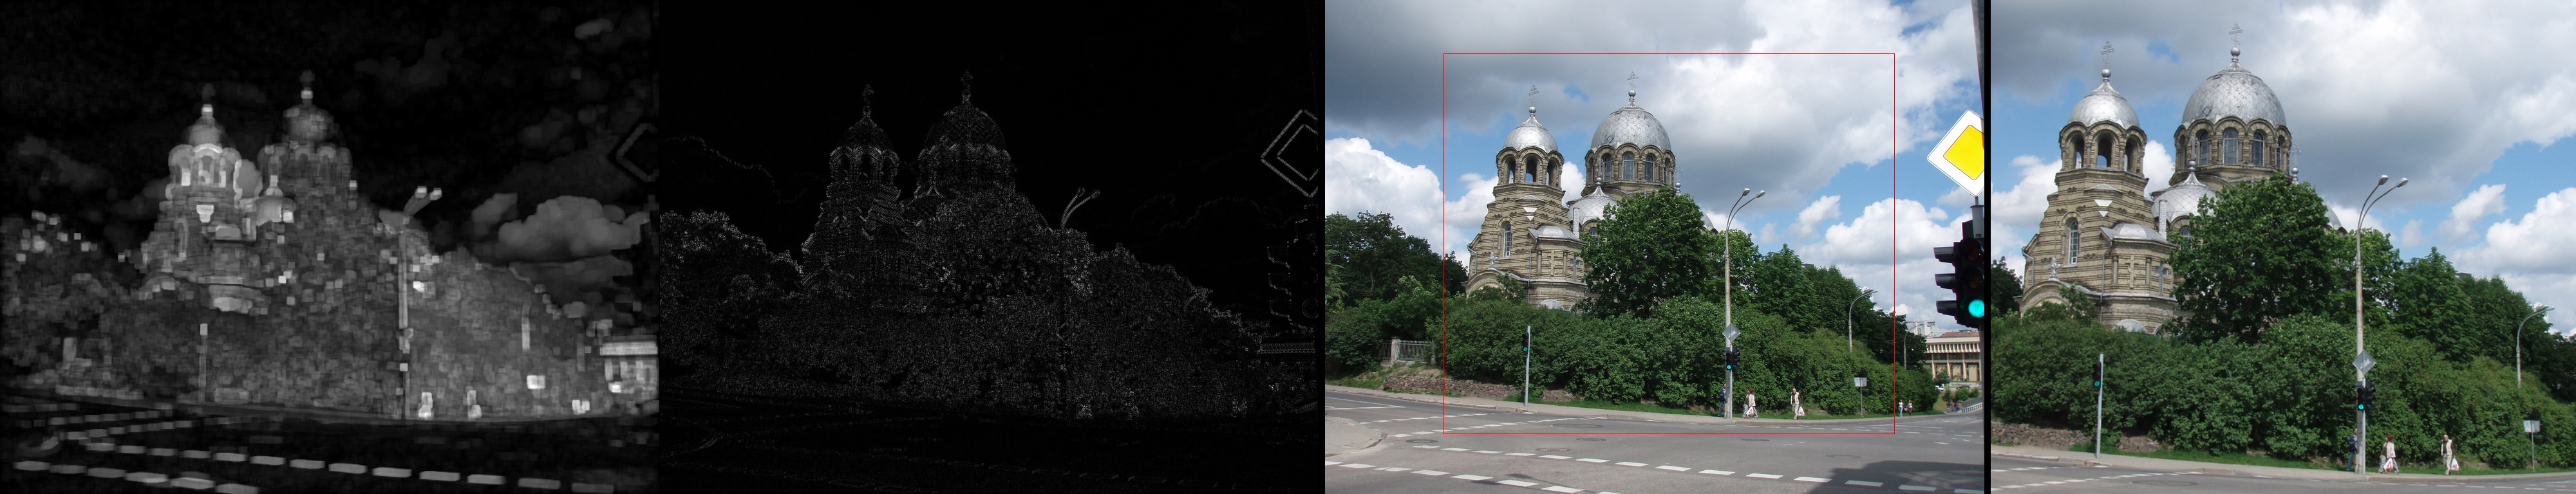
\includegraphics[width=11.5cm]{../figures/example_autocrop.jpg}
\end{figure}
\begin{enumerate}
	\item Saliency Composition
	\item Boundary Simplicity
	\item Content Preservation
\end{enumerate}
\clearpage

\ETHminimal
\textbf{Method: Cropping - Features}
\begin{itemize}
	\item Saliency composition
		\begin{itemize}
		\item 3-level spatial pyramid of saliency map
		\item $4^2 + 2^2 + 1 = 21$ features.
		\end{itemize}
	\item Boundary simplicity
		\begin{itemize}
		\item Gradient map generated using Sobel filter and \texttt{abs}.
		\item Mean value of 2-pixel wide strips used.
		\item $4$ features, $1$ per edge.
		\end{itemize}
	\item Content preservation
		\begin{itemize}
		\item Sum of all salient energy in crop
		\end{itemize}
\end{itemize}
\clearpage

\ETHminimal
\textbf{Method: Cropping - Datasets}
\begin{itemize}
	\item Human crop dataset
		\begin{itemize}
		\item Collected from Amazon Mechanical Turks, Chen et al. (2014)
		\item 500 images, 10 crops per image.
		\item Used for evaluating model.
		\end{itemize}
	\item Reddit dataset
		\begin{itemize}
		\item Top 2000 images in the past year.
		\item Subreddits used: \tiny{CityPorn, EarthPorn, itookapicture, photocritique, WaterPorn, windowshots}\normalsize
		\item Used for training model.
		\end{itemize}
\end{itemize}
\begin{tikzpicture}[remember picture,overlay]
  \node [xshift=-6cm,yshift=-8.6cm] at (current page.north east)
    {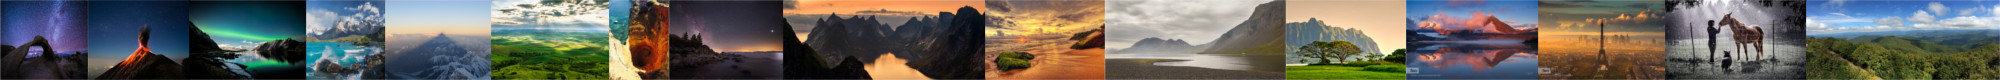
\includegraphics[width=14.4cm]{../figures/example_reddit.jpg}};
\end{tikzpicture}
\clearpage

\ETHminimal
\textbf{Method: Cropping - Final\\}
\newline
\begin{minipage}{0.4\textwidth}
\vskip3.6cm
\scriptsize
\begin{gather*}
	S_{content} = \frac{\mathrm{sum(cropped\ saliency)}}{\mathrm{sum(full\ saliency)}}
\end{gather*}
$\cdot$ Start from large crops. \\
$\cdot$ Find smaller crops. \\
$\cdot$ Stop when enough candidates.
\end{minipage}
\begin{tikzpicture}[remember picture,overlay]
  \node [xshift=-3.9cm,yshift=-4.8cm] at (current page.north east)
    {\includegraphics[width=6.5cm]{../figures/pipeline_cropfinal.pdf}};
\end{tikzpicture}
\clearpage

\ETHminimal
\textbf{Final pipeline}
\begin{figure}[h!]
\centering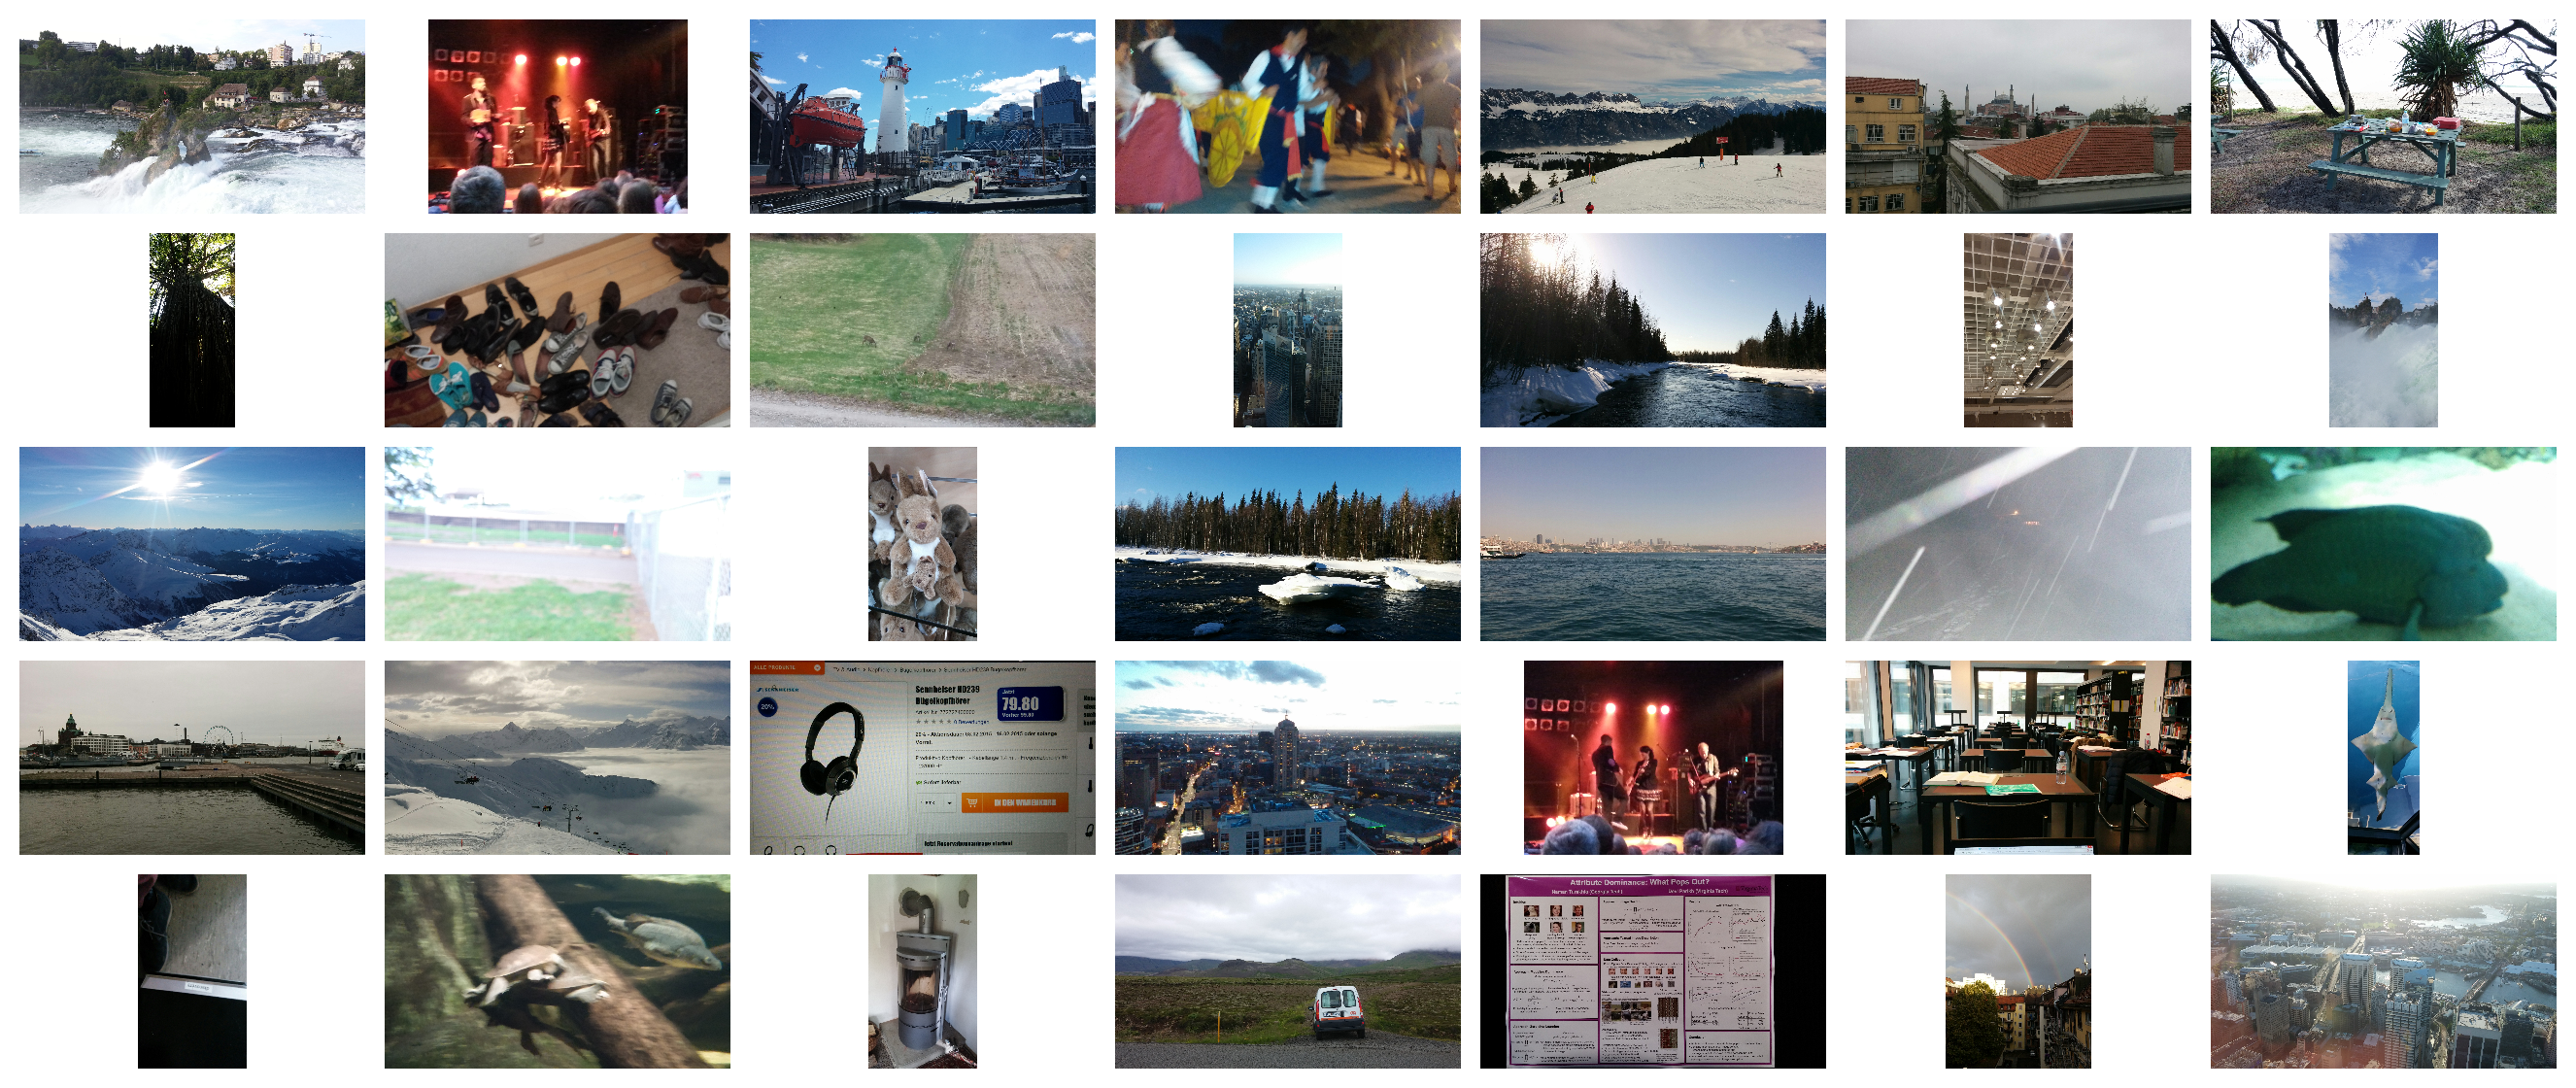
\includegraphics[width=11.5cm]{../figures/grid5x7_out1.png}
\end{figure}
\clearpage

\ETHminimal
\textbf{Final pipeline}
\begin{figure}[h!]
\centering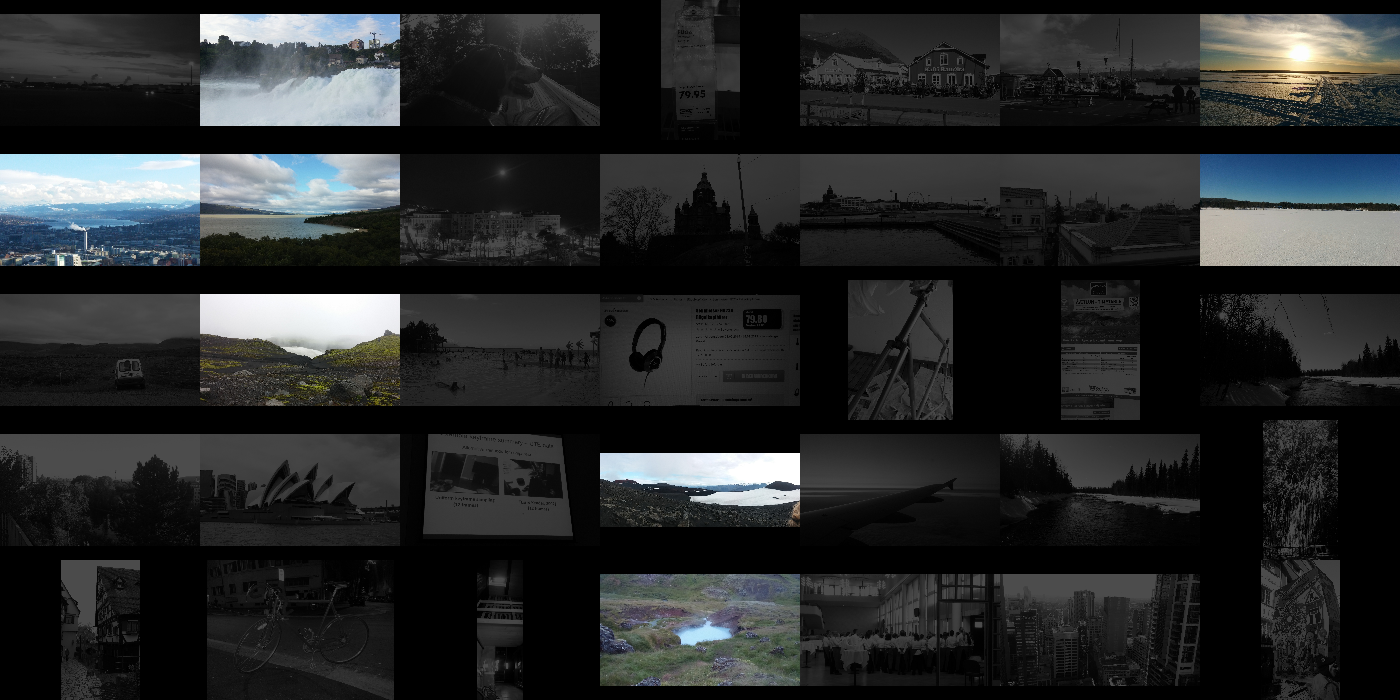
\includegraphics[width=11.5cm]{../figures/grid5x7_out2.png}
\end{figure}
\clearpage

\ETHminimal
\textbf{Final pipeline}
\begin{figure}[h!]
\centering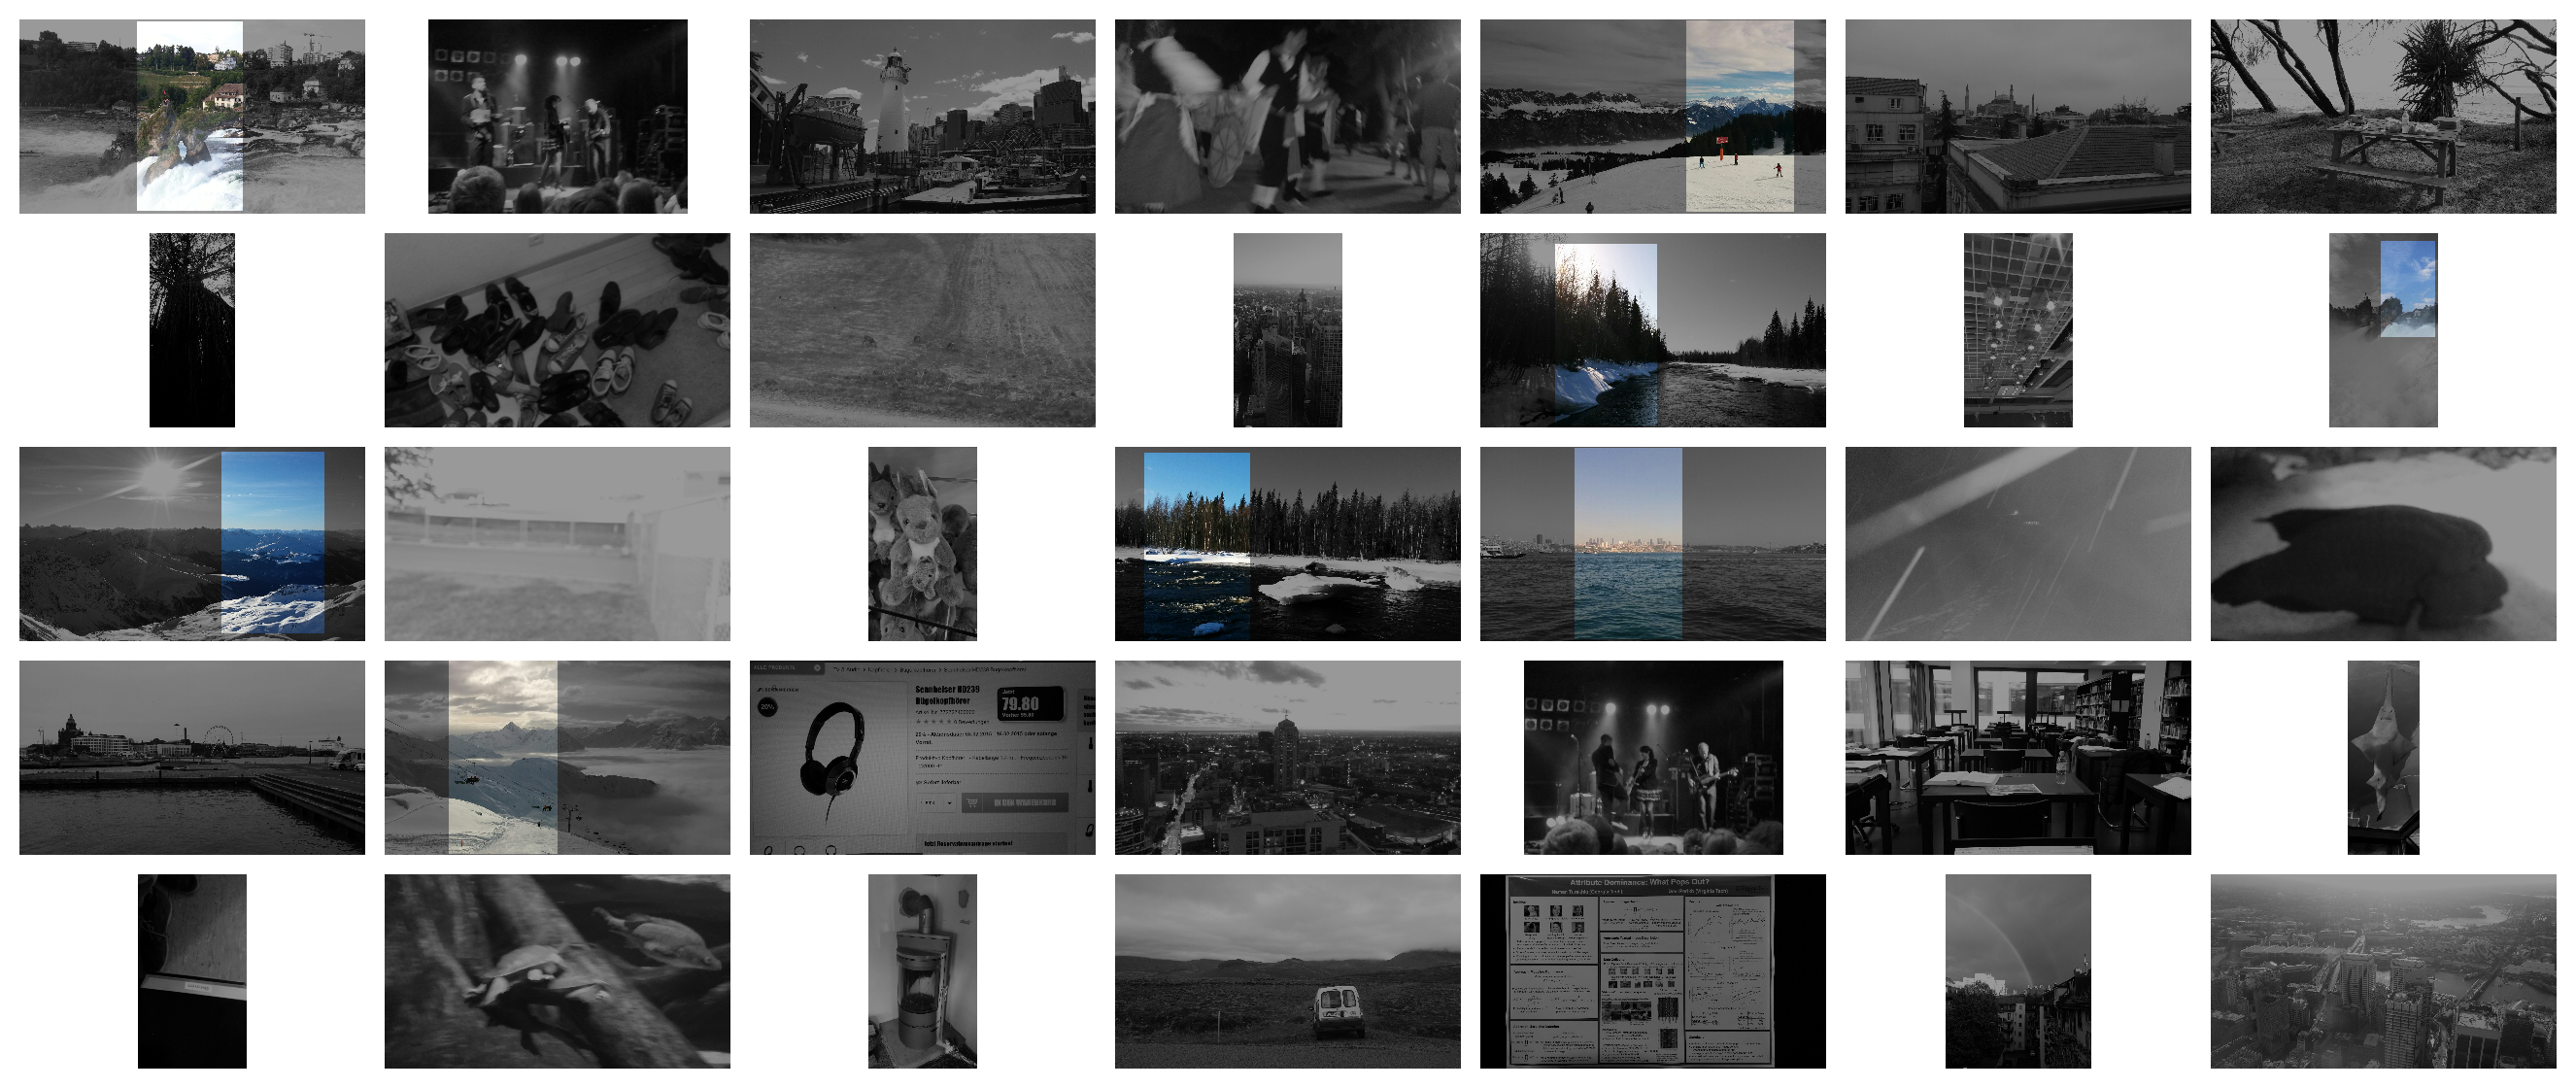
\includegraphics[width=11.5cm]{../figures/grid5x7_out3.png}
\end{figure}
\clearpage

\ETHminimal
\textbf{Results: Suitability\\}
\begin{itemize}
	\item Top 7 suitable images from Michael dataset.
	\item Suitability decreases towards right.
	\item 53 suitable images left out of 275.
	\item Favours distant natural scenes.
\end{itemize}
\begin{tikzpicture}[remember picture,overlay]
  \node [xshift=-6.4cm,yshift=-7.0cm] at (current page.north east)
    {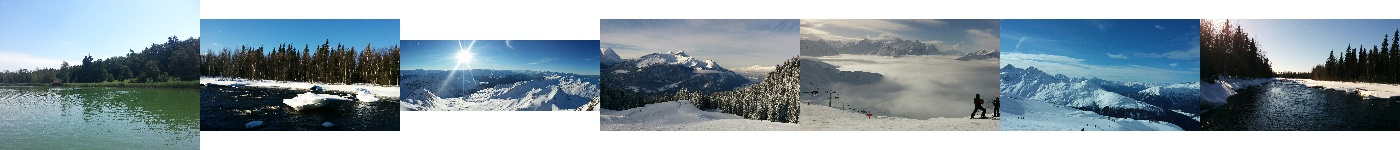
\includegraphics[width=12.9cm]{../figures/top7_suitable.jpg}};
\end{tikzpicture}
\clearpage

\ETHminimal
\textbf{Analysis: Suitability}
\begin{itemize}
	\item Classifications gathered from four people. (\% marked as suitable)
	\begin{itemize}
		\item Michael set: $48\%$, $37\%$, $31\%$, $63\%$
		\item Wookie set: $23\%$, $20\%$, $17\%$, $37\%$
	\end{itemize}
	\item Pearson correlation coeff between two classification sets is \\ 0.51 (Michael), 0.23 (Wookie)
	\item When considering images with classifications in consensus:
	\begin{itemize}
		\item Trained on Wookie set: $9.8\%$ error.
		\item Trained on Michael set: $12.4\%$ error.
	\end{itemize}
\end{itemize}
\clearpage

\ETHminimal
\textbf{Results: Cropping (Good)}
\begin{figure}[h!]
\centering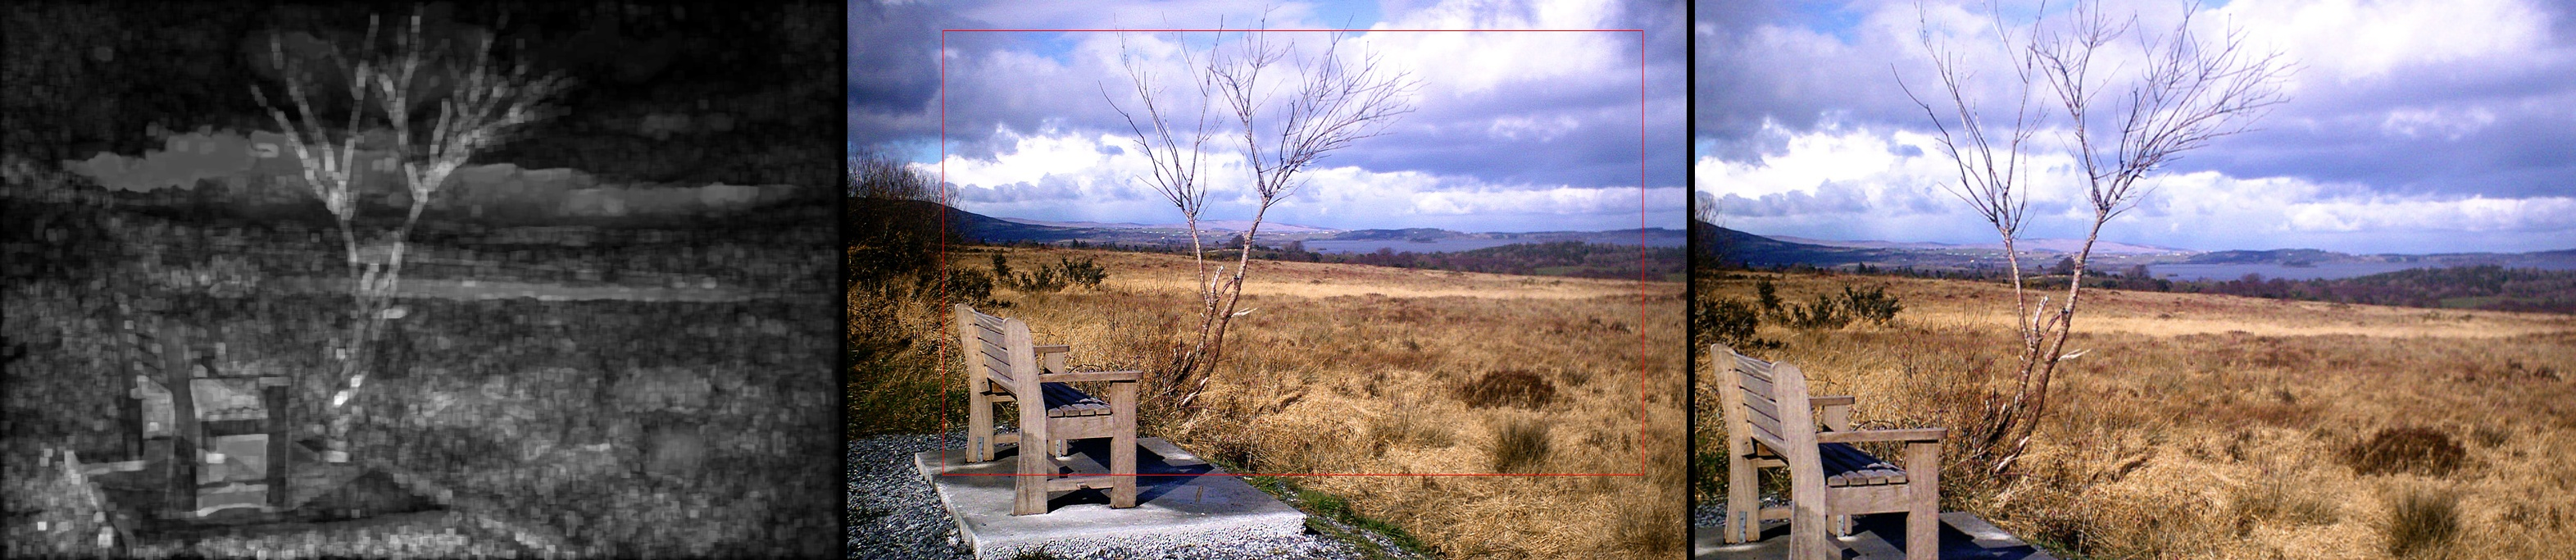
\includegraphics[width=11.5cm]{../figures/good_crops/109123697_Large.jpg}
\vskip2mm
\centering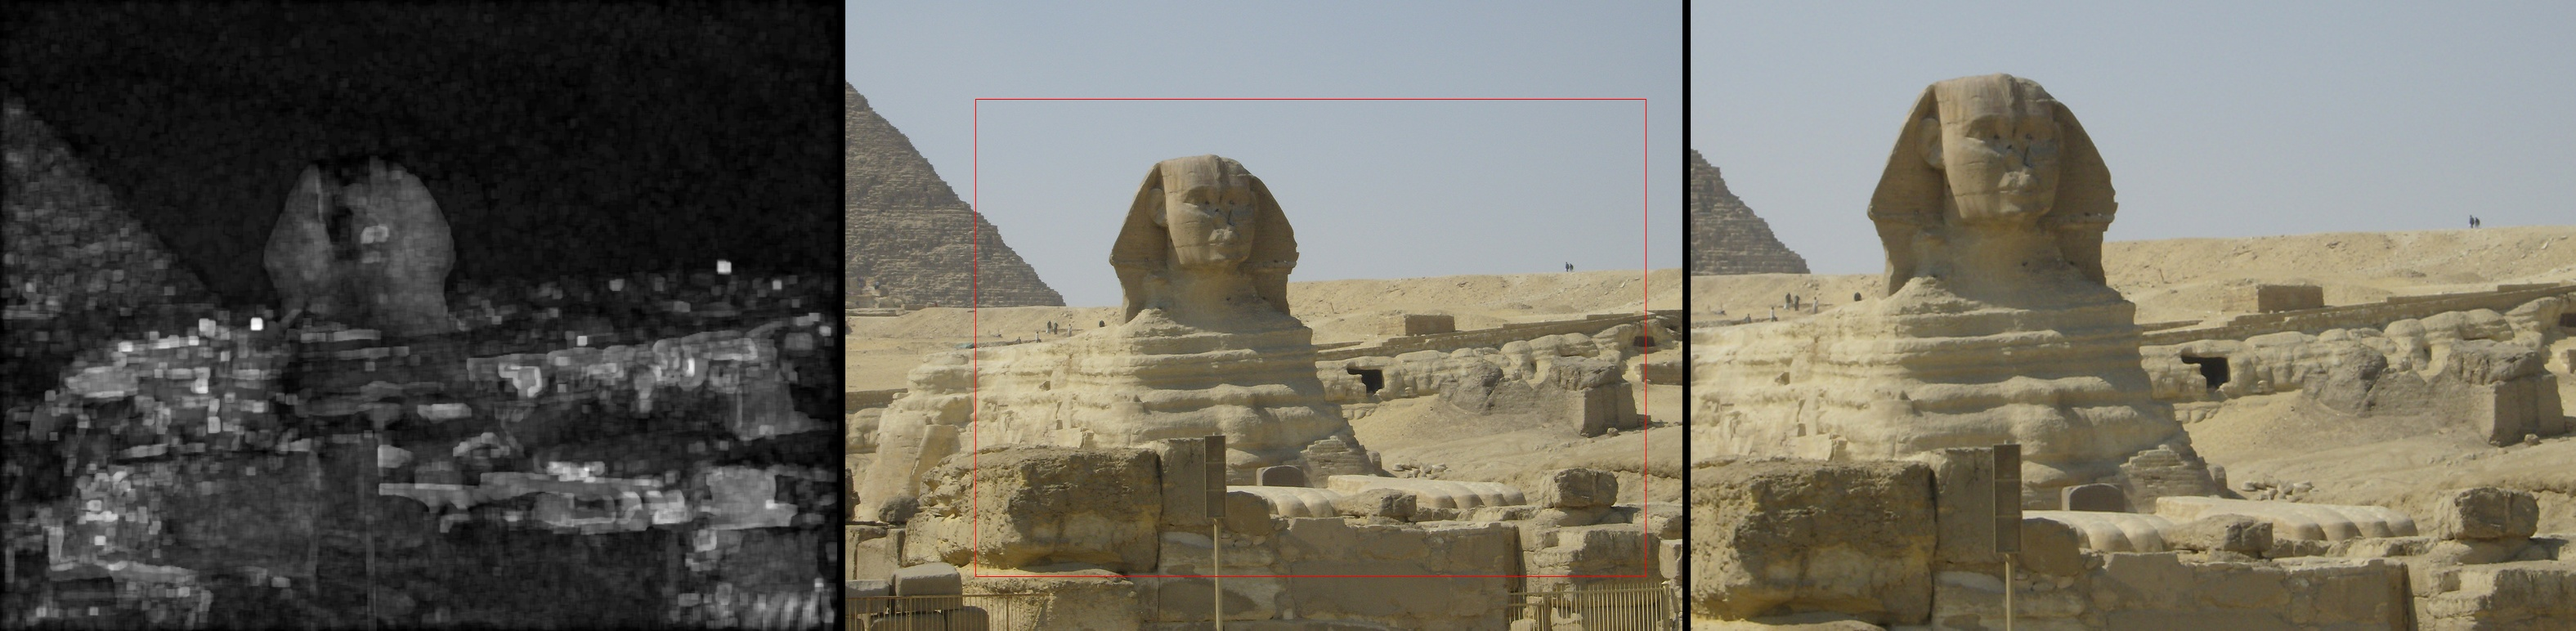
\includegraphics[width=11.5cm]{../figures/good_crops/1158647496_Large.jpg}
\end{figure}
\clearpage

\ETHminimal
\textbf{Results: Cropping (Good)}
\begin{figure}[h!]
\centering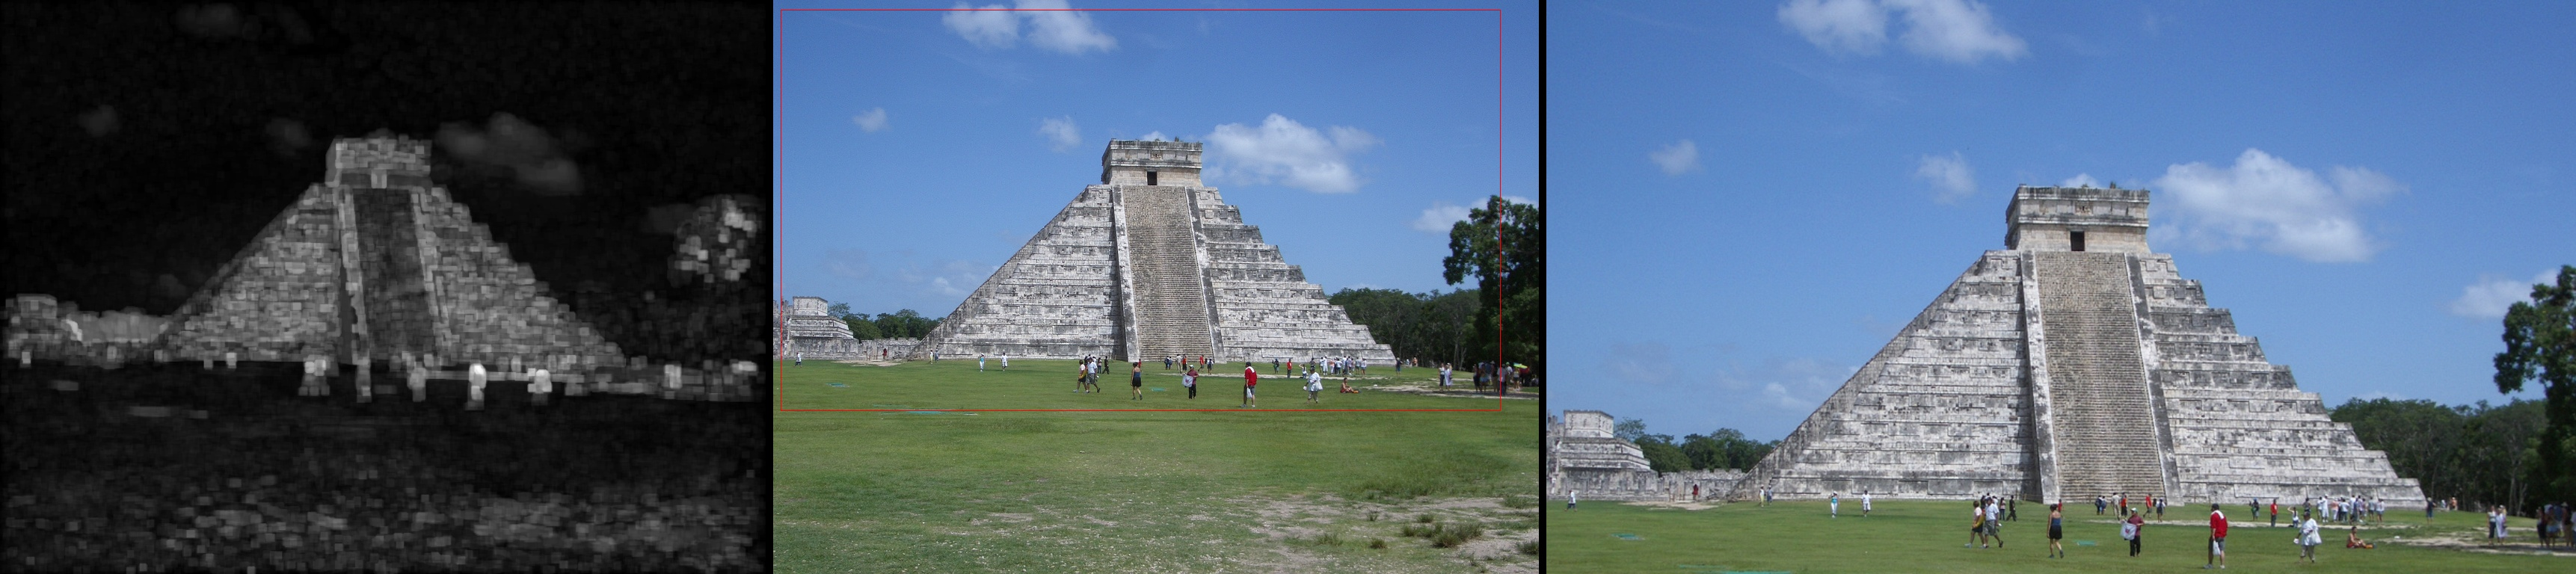
\includegraphics[width=11.5cm]{../figures/good_crops/236441280_Large.jpg}
\vskip2mm
\centering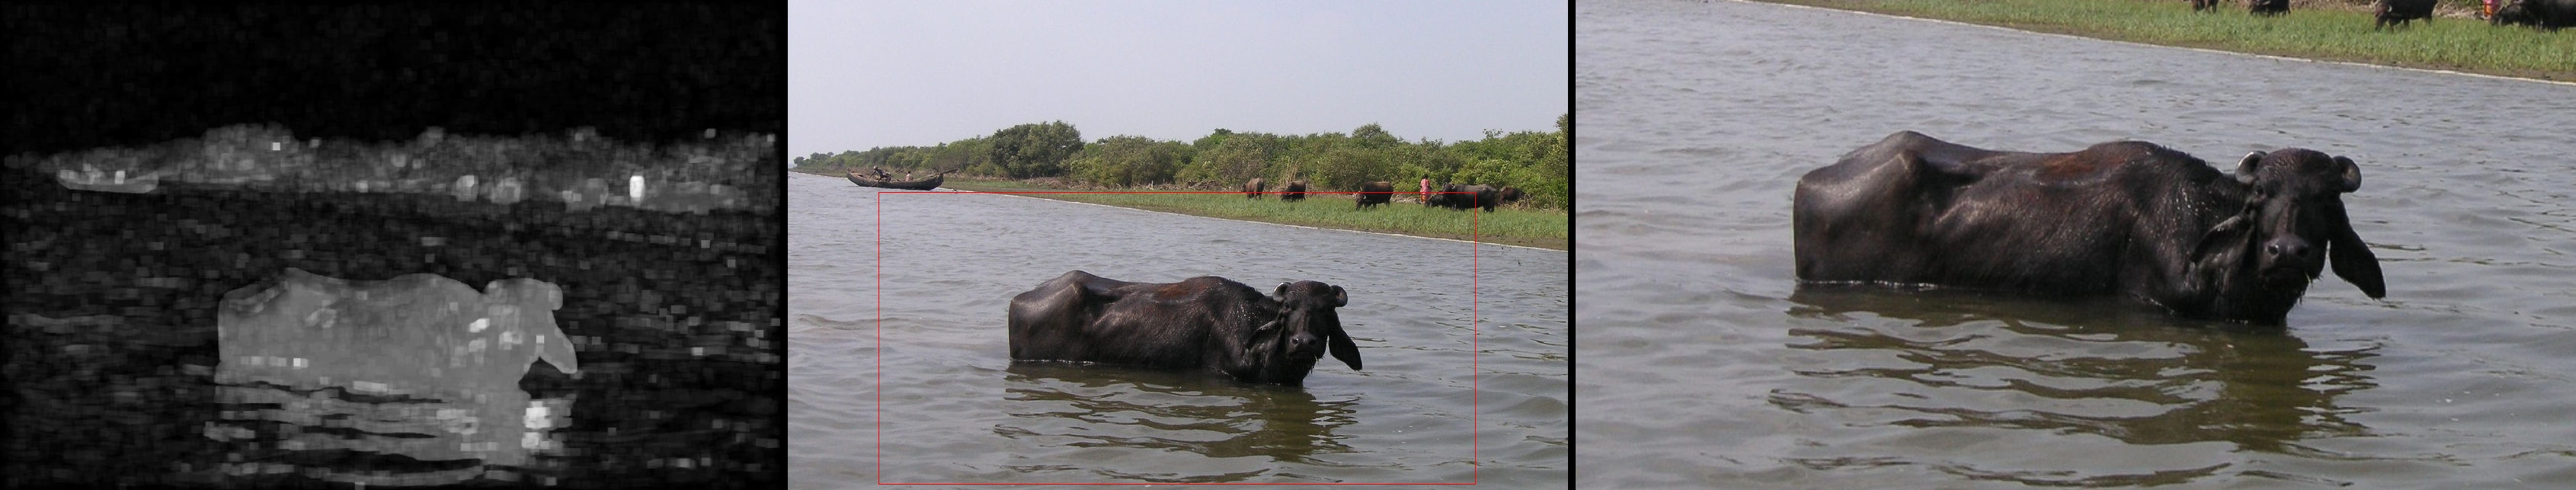
\includegraphics[width=11.5cm]{../figures/good_crops/371485783_Large.jpg}
\end{figure}
\clearpage

\ETHminimal
\textbf{Results: Cropping (Good)}
\begin{figure}[h!]
\centering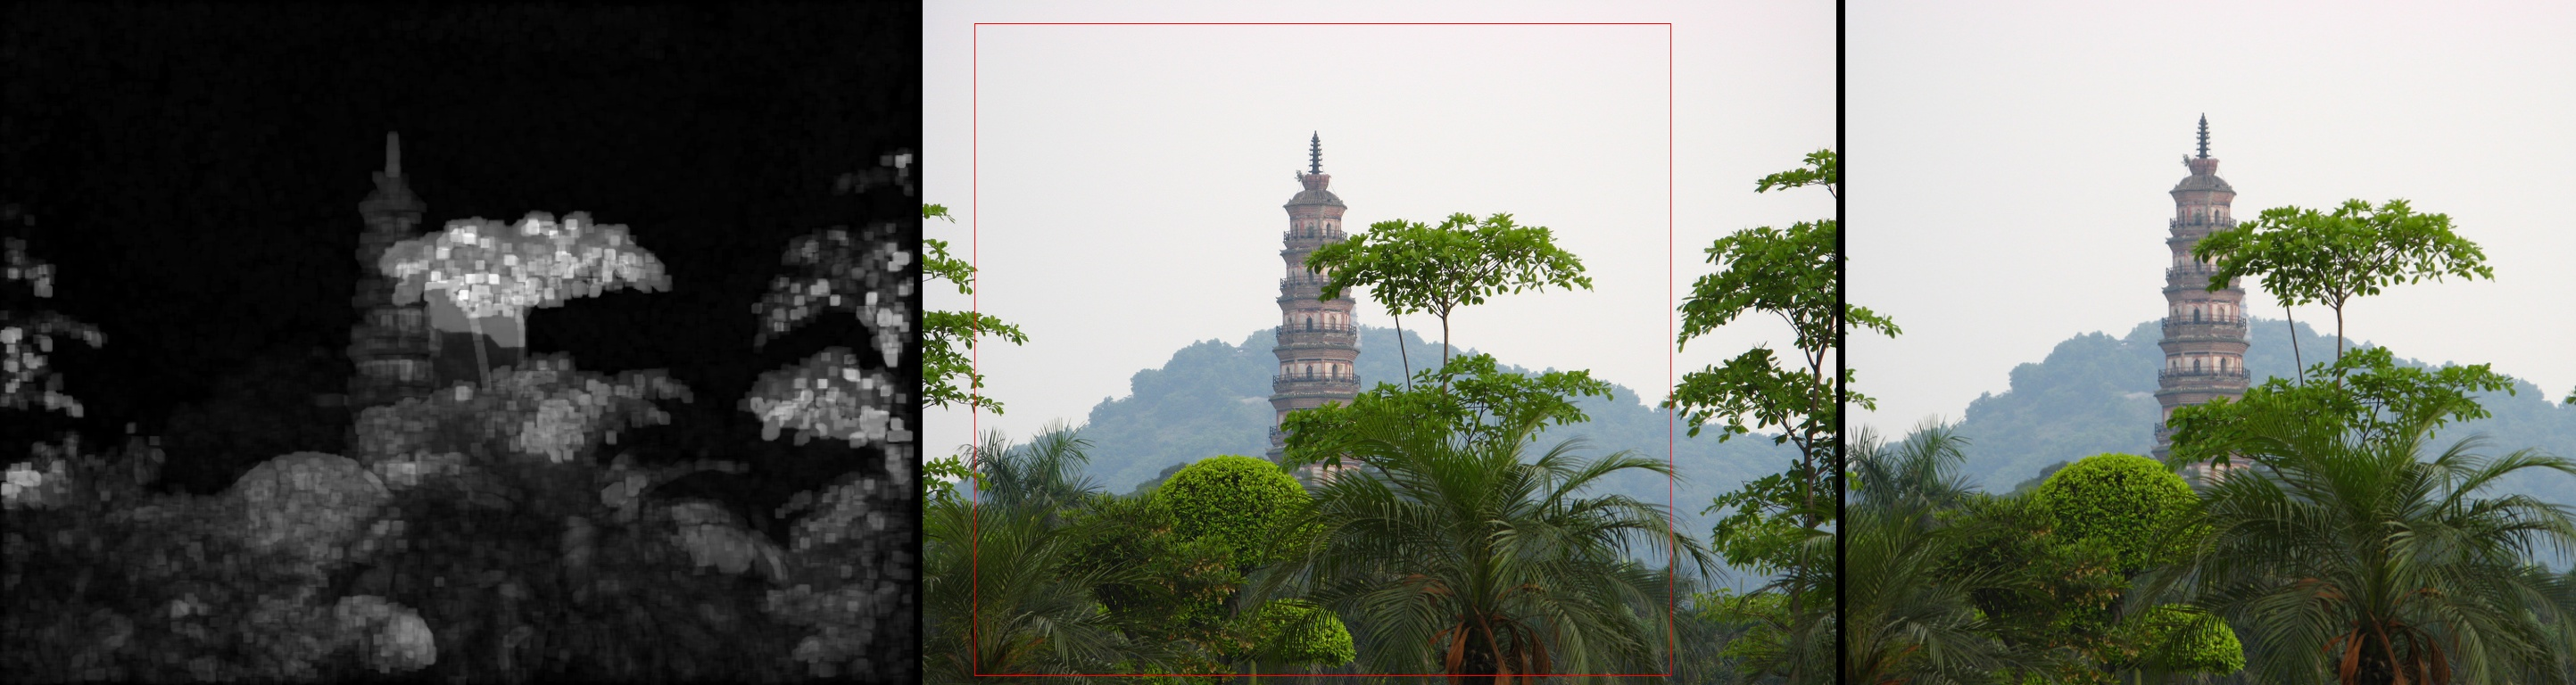
\includegraphics[width=11.5cm]{../figures/good_crops/504325680_Large.jpg}
\vskip2mm
\centering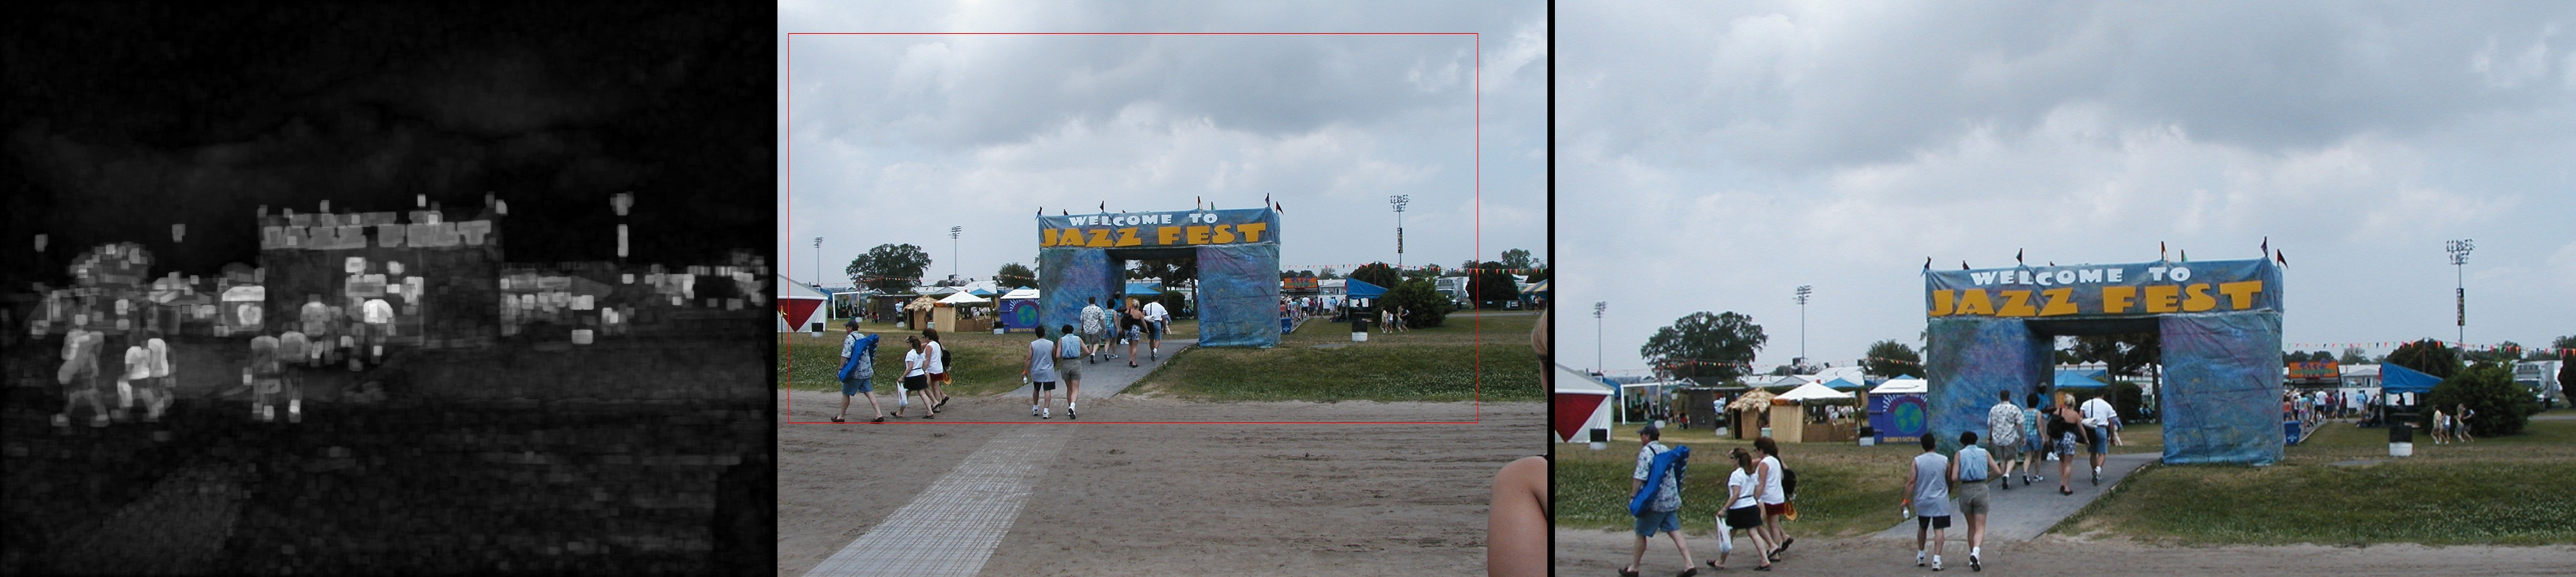
\includegraphics[width=11.5cm]{../figures/good_crops/52968615_Large.jpg}
\end{figure}
\clearpage


\ETHminimal
\textbf{Results: Cropping (Bad)}
\begin{figure}[h!]
\centering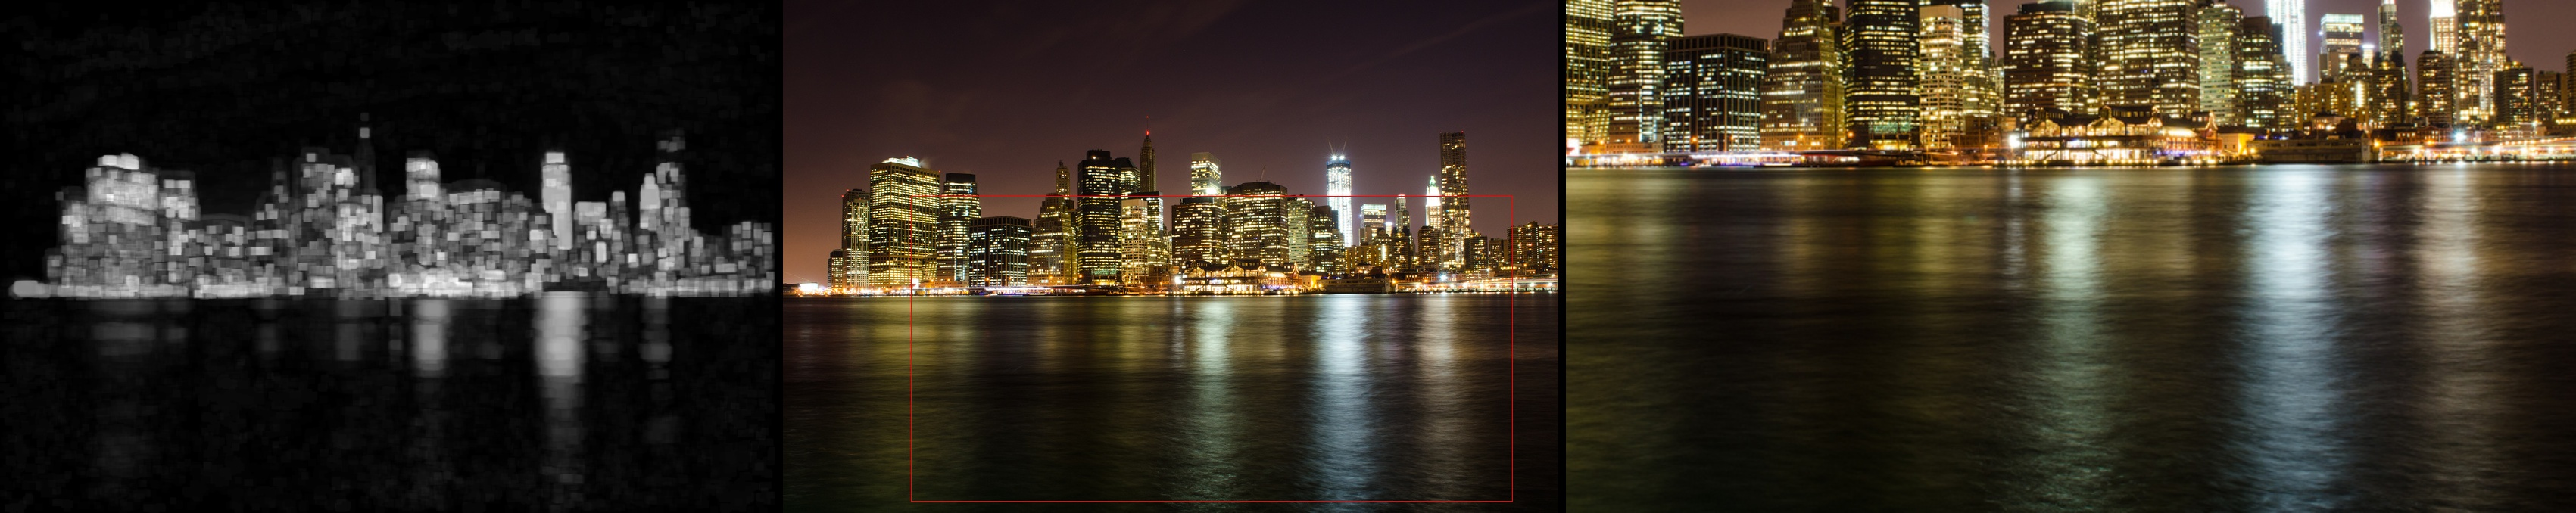
\includegraphics[width=11.5cm]{../figures/bad_crops/6857081990_Large.jpg}
\vskip2mm
\centering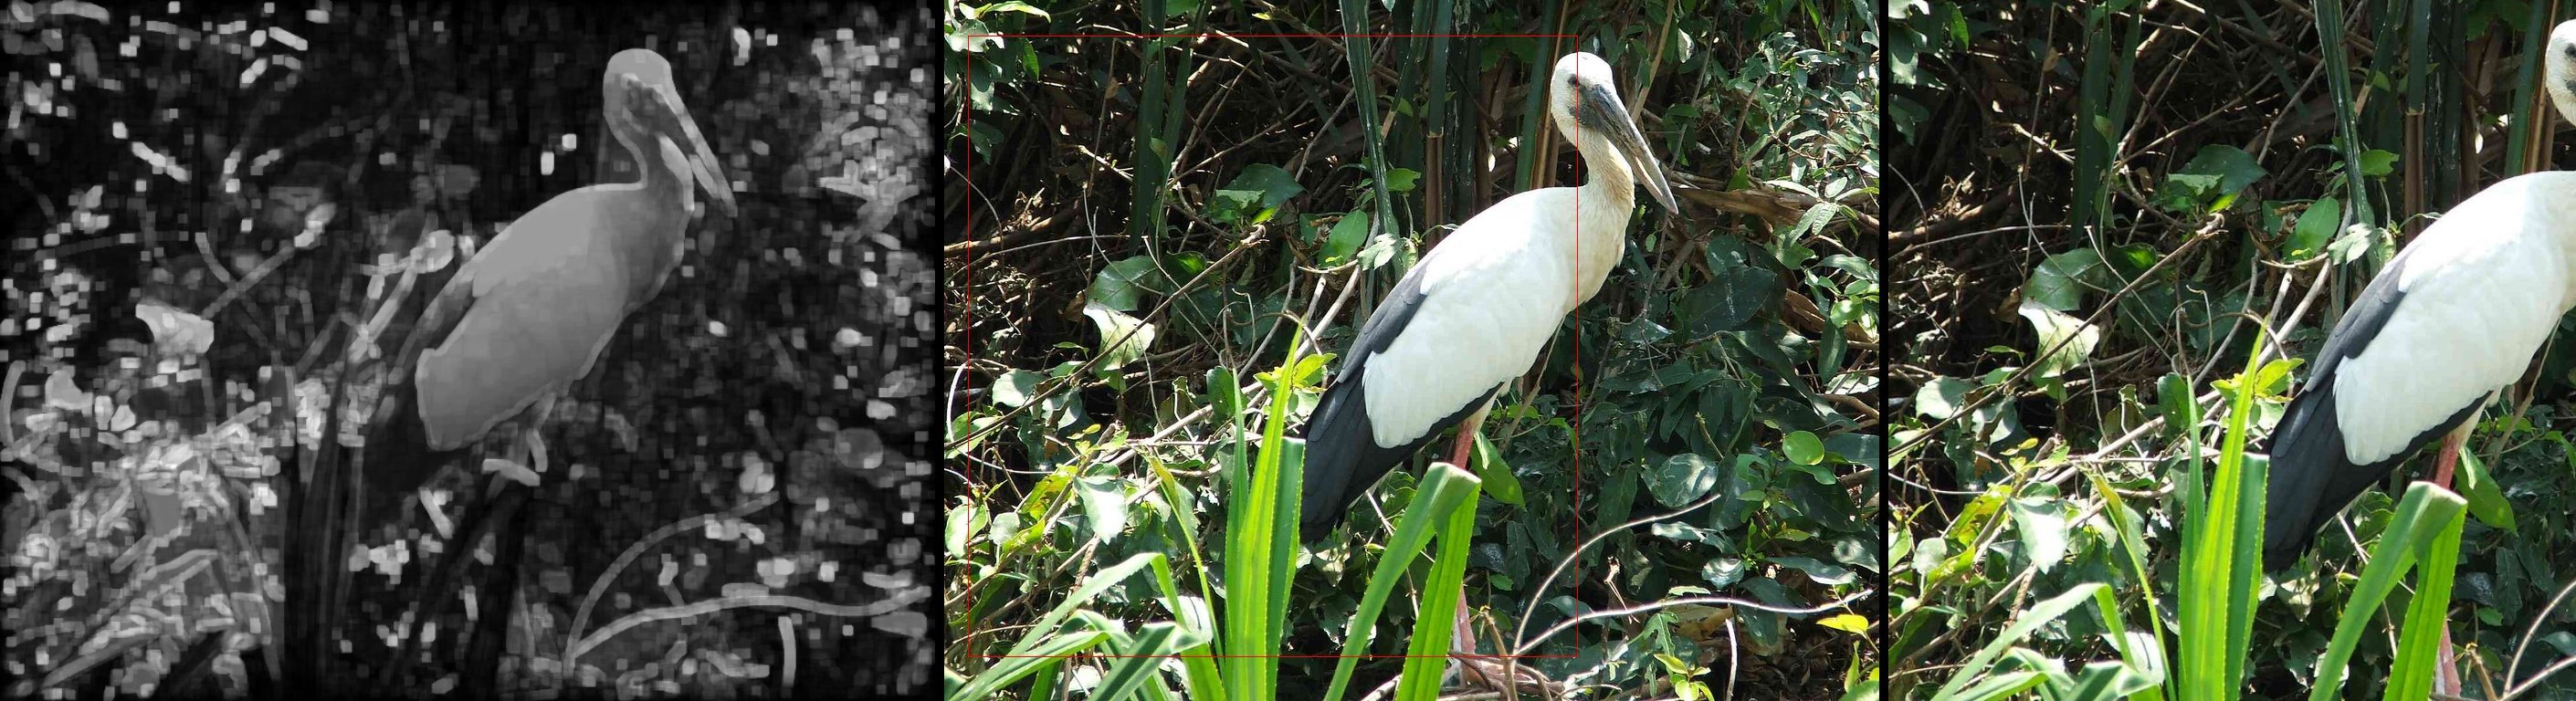
\includegraphics[width=11.5cm]{../figures/bad_crops/118697470_Large.jpg}
\end{figure}
\clearpage

\ETHminimal
\textbf{Analysis: Cropping\\}
\newline
\begin{gather*}
	\mathrm{Overlap}(C_i, H_j) = \frac{C_i \cap H_j}{C_i \cup H_j} \\
	\mathrm{MaxOverlap}(C_i, H) = \max_j\mathrm{Overlap}(C_i, H_j)
\end{gather*}
\begin{itemize}
	\item $C_i$ is the $i$-th crop candidate, and
	\item $H_j$ is the $j$-th human crop. There are $10$ human crops per image.
	\item $\mathrm{MaxOverlap}$ is calculated for $i\in\{1, 2, 3, 4, 5\}$.
	\item $C_1$ is the highest scoring crop.
\end{itemize}
\clearpage

\ETHminimal
\textbf{Analysis: Cropping\\}
\begin{minipage}{0.5\textwidth}
\vskip5.5cm
\footnotesize{
	Improvements: \\
	$\cdot$ 4 Boundary features \\
	$\cdot$ Saliency sum feature \\
	$\cdot$ Shrinking content threshold
}
\end{minipage}

\begin{tikzpicture}[remember picture,overlay]
  \node [xshift=-4.5cm,yshift=-5.1cm] at (current page.north east)
    {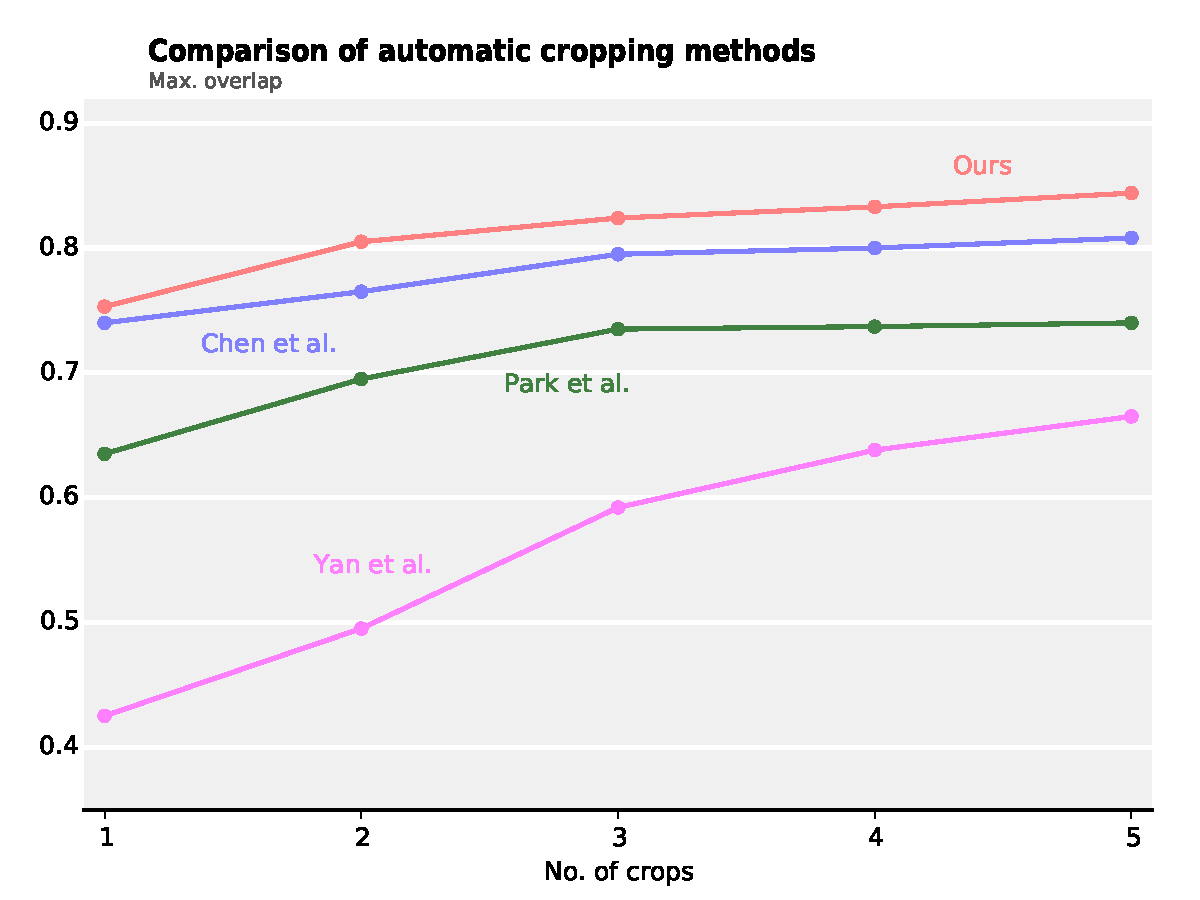
\includegraphics[width=9cm]{../figures/comparison.pdf}};
\end{tikzpicture}
\clearpage

\ETHminimal
\textbf{Summary\\}
\begin{itemize}
	\item Trained models to select and crop an image given a set of images.
	\item Suitability classification error of $9.8\%$.
	\item Improved cropping algorithm.\\ First 5 crop yields max. overlap of 0.84 over 0.81 from Chen et al.
	\vskip1cm
	\item Implementation in \texttt{C++} (Cropping) and \texttt{Python} (Suitability) using OpenCV and Caffe.
\end{itemize}
\clearpage

\ETHminimal
\textbf{Further Work\\}
\begin{itemize}
	\item Suitability
	\begin{itemize}
		\item Train on larger datasets with wide range of objects.
		\item Add features for image quality and colour distribution.
		\item Reduce classification bias.
	\end{itemize}

	\item Cropping
	\begin{itemize}
		\item Try different saliency map implementations.
		\item Find other visual cues such as variance of salient energy.
	\end{itemize}
\end{itemize}
\clearpage

\end{document}
